\documentclass{jhwhw}

\title{HCI 9649 JCI MYE}
\author{Eytan Chong}
\date{2024-06-03}

\begin{document}
    \problem{}
        \textbf{Omitted.}

    \problem{}
        A point $P$ lies on the curve $C$ with polar equation $r = 2a\cos\theta$, $-\dfrac\pi2 < \theta \leq \dfrac\pi2$, where $a$ is a positive constant. The point $N$ is the foot of the perpendicular from the pole to the tangent of $C$ at $P$.

        \begin{enumerate}
            \item Sketch $C$, $P$ and $N$ on the same diagram.
            \item By considering the polar coordinates of $N$, show that, as $P$ varies, the locus of $N$ is given by the polar equation $r = a(1 + \cos\theta)$, $-\pi < \theta \leq \pi$.
        \end{enumerate}

    \solution
        \part
            \begin{center}
                \begin{tikzpicture}
                    \coordinate[label=left:$O$] (O) at (0, 0);
                    \coordinate[label=below:$A\coord{0}{a}$] (A) at (3, 0);
                    \coordinate[label=above right:$P$] (P) at (9/2, 2.6);
                    \coordinate[label=above right:$N$] (N) at (2.249, 3.899);
                    \coordinate[label=below:$B$] (B) at (9.006, 0);
                    \coordinate[label=below right:$C$] (C) at (9/2, -2.6);

                    \draw[->] (O)--(10.5, 0) node[anchor=south east] {$\theta = 0$};
                    \draw (A) circle[radius=3];
                    \draw (0, 5.196)--(B);
                    \draw (A)--(P);
                    \draw (O)--(P);
                    \draw (O)--(N);

                    \draw pic [draw, angle radius=12mm, "$\theta$"] {angle = A--O--P};
                    \draw pic [draw, angle radius=14mm, "$\varphi$"] {angle = P--O--N};
                    \draw pic [draw, angle radius=12mm, "$2\theta$"] {angle = B--A--P};
                    \draw pic [draw, angle radius=3mm, ""] {right angle = O--N--P};
                    \draw pic [draw, angle radius=3mm, ""] {right angle = A--P--B};
                \end{tikzpicture}
            \end{center}

        \part
            Consider the diagram above. Let $N(\theta + \varphi, r)$. Let $B$ be the intersection between the tangent at $P$ and the half-line $\theta = 0$. Note that $C$ is a circle centered at $A$ with radius $a$.

            Since angle at centre is twice angle at circumference, $\angle PAB = 2\angle POA = 2\theta$. Since tangent to circle is parallel to radius, $AP \perp PB$. Hence, $ON \parallel AP \implies \angle NOA = \angle PAB \implies \varphi = \theta$.

            Since $\cos\angle NOP = \dfrac{ON}{OP}$, we have
            \begin{align*}
                ON &= OP\cos\theta\\
                &= (2a\cos\theta)\cos\theta\\
                &= 2a\cos^2\theta\\
                &= a\left(2\cos^2\theta - 1 + 1\right)\\
                &= a(\cos2\theta + 1)
            \end{align*}

            Hence, $N(\theta + \varphi, r) = \Big(2\theta, a(\cos2\theta + 1)\Big) = \Big(\theta, a(\cos\theta + 1)\Big)$. Thus, the locus of $N$ is given by $r = a(1 + \cos\theta)$.

    \problem{}
        The sequence $\{u_n\}$ is given by the recurrence relation
        \begin{equation*}
            u_{n+2} = 5u_{n+1} - 6u_n, \, n \in \mathbb{Z}^+
        \end{equation*}
        together with terms $u_1 = a$ and $u_2 = b$.

        \begin{enumerate}
            \item Find the expression of $u_n$ in terms of $a$ and $b$.
            \item Find algebraically the possible limits of $\dfrac{u_n}{u_{n-1}}$.
        \end{enumerate}

    \solution
        \part
            Consider the characteristic equation of the recurrence relation.
            \begin{alignat*}{2}
                &&x^2 - 5x + 6 &= 0\\
                \implies&&(x-2)(x-3) &= 0
            \end{alignat*}
            Hence, the roots of the characteristic equation are 2 and 3. Thus,
            \begin{equation*}
                u_n = A\cdot2^n + B\cdot3^n
            \end{equation*}
            Substituting $n = 1$ and $n=2$, we have
            \begin{equation*}
                \systeme[AB]{2A + 3B = a, 4A + 9B=b}
            \end{equation*}
            which has solution $A = \dfrac{3a-b}2$ and $B = \dfrac{b-2a}3$. Thus,
            \boxt{
                $u_n = \dfrac{3a-b}2\cdot2^n + \dfrac{b-2a}3\cdot3^n$
            }

        \part
            Let $L = \lim\limits_{n \to \infty} \dfrac{u_n}{u_{n-1}}$.
            \begin{alignat*}{2}
                &&u_{n+2} &= 5u_{n+1} - 6u_{n}\\
                \implies&&\dfrac{u_{n+2}}{u_{n+1}} &= 5 - 6 \cdot \dfrac{u_{n}}{u_{n+1}}\\
                \implies&&\lim_{n \to \infty}\dfrac{u_{n+2}}{u_{n+1}} &= \lim_{n \to \infty}\left(5 - 6 \cdot \dfrac{u_{n}}{u_{n+1}}\right)\\
                \implies&& L &= 5 - \dfrac6L\\
                \implies&&L^2 -5L + 6 &= 0\\
                \implies&&(L-2)(L-3) &= 0\\
                \implies&&L &= 2 \lor 3
            \end{alignat*}
            \boxt{
                The possible limits are 2 and 3.
            }

    \problem{}
        \textbf{Omitted.}

    \problem{}
        The points $A$ and $B$ have Cartesian coordinates $\coord{a}0$ and $\coord{-a}0$ respectively, where $a$ is a positive constant. The point $P$ is such that $AP \cdot BP = a^2$. The curve $C$ describes the locus of $P$.

        \begin{enumerate}
            \item Show that $C$ has polar equation $r^2 = 2a^2\cos2\theta$, $0 \leq \theta \leq 2\pi$.
            \item Sketch the graph of $C$, indicating all key features and symmetries of the curve.
            \item Find the exact area of the region enclosed by the curve $C$.
        \end{enumerate}

    \solution
        \part
            Let $P\coord{x}{y}$.
            \begin{alignat*}{2}
                &&AP \cdot BP &= a^2\\
                \implies&&AP^2 \cdot BP^2 &= a^4\\
                \implies&&\Big((x-a)^2 + y^2\Big)\Big((x+a)^2 + y^2\Big) &= a^4\\
                \implies&&(x-a)^2(x+a)^2 + y^2(x+a)^2 + y^2(x-a)^2 + y^4 &= a^4\\
                \implies&&\left(x^2 - a^2\right)^2 + y^2\Big((x+a)^2 + (x-a)^2\Big) + y^4&= a^4\\
                \implies&&\left(x^4 -2a^2x^2 + a^4\right) + y^2\Big(\left(x^2 + 2ax + a^2\right) + \left(x^2 - 2ax + a^2\right)\Big) + y^4&= a^4\\
                \implies&&x^4 -2a^2x^2 + 2y^2\Big(x^2 + a^2\Big) + y^4 &= 0\\
                \implies&&x^4 -2a^2x^2 + 2x^2y^2 + 2a^2y^2 + y^4 &= 0\\
                \implies&&\left(x^4  + 2x^2y^2 + y^4\right) + \left(2a^2y^2 -2a^2x^2\right)&= 0\\
                \implies&&\left(x^2 + y^2\right)^2 + 2a^2\left(y^2 - x^2\right)&= 0\\
                \implies&&\left(r^2\right)^2 + 2a^2\left((r\sin\theta)^2 - (r\cos\theta)^2\right)&= 0\\
                \implies&&r^4 + 2a^2r^2\left(\sin^2\theta - \cos^2\theta\right)&= 0\\
                \implies&&r^4 - 2a^2r^2\cos2\theta&= 0\\
                \implies&&r^2 - 2a^2\cos2\theta&= 0\\
                \implies&&r^2 &= 2a^2\cos2\theta
            \end{alignat*}

        \part
            \begin{center}
                \begin{tikzpicture}[trim axis left, trim axis right]
                    \begin{axis}[
                        samples = 1000,
                        axis y line=middle,
                        axis x line=middle,
                        xtick = \empty,
                        ytick = \empty,
                        xmin=-1.5,
                        xmax=1.5,
                        ymin=-1.5,
                        ymax=1.5,
                        xlabel = {$\theta=0$},
                        ylabel = {$\theta = \frac\pi2$},
                        legend cell align={left},
                        legend pos=outer north east,
                        after end axis/.code={
                            \path (axis cs:0,0) 
                                node [anchor=north east] {$O$};
                            }
                        ]
                        \addplot[color=plotRed,data cs=polarrad, domain=-pi/2:pi/2] {sqrt(2*cos(2*\x r))};

                        \addplot[color=plotRed,data cs=polarrad, domain=pi/2:3*pi/2] {sqrt(2*cos(2*\x r))};
            
                        \addlegendentry{$C$};

                        \addplot[dotted] {x};
                        \addplot[dotted] {-x};

                        \node[anchor=east] at (1.414, 1.31) {$\theta = \frac14 \pi$};

                        \node[anchor=west] at (-1.414, 1.31) {$\theta = \frac34 \pi$};

                        \node[anchor=west] at (-1.414, -1.31) {$\theta = \frac54 \pi$};

                        \node[anchor=east] at (1.414, -1.31) {$\theta = \frac74 \pi$};
                    \end{axis}
                \end{tikzpicture}
            \end{center}

        \part
            \begin{align*}
                \text{Area} &= 2 \cdot \dfrac12 \int_{-\pi/4}^{\pi/4} r^2 \d \theta\\
                &= \int_{-\pi/4}^{\pi/4} 2a^2\cos2\theta \d \theta \usub{u &= 2\theta\\du &= 2 \d \theta}\\
                &= a^2 \int_{-\pi/2}^{\pi/2} \cos u \d u\\
                &= a^2 \eval{\sin u}{-\pi/2}{\pi/2}\\
                &= 2a^2
            \end{align*}

            \boxt{
                The area of the region enclosed by $C$ is $2a^2$ units$^2$.
            }

    \problem{}
        In the diagram, the curve with equation $2y = 1 + \ln x$ for $x > 0$ divides the rectangle bounded by the axes, the lines $y = 1$ and $x = e$ into two regions, $S$ and $T$.

        \begin{center}
            \begin{tikzpicture}[trim axis left, trim axis right]
                \begin{axis}[
                    domain = 0:10,
                    samples = 101,
                    axis y line=middle,
                    axis x line=middle,
                    xtick = {2.718},
                    xticklabels = {$e$},
                    ytick = {1},
                    xlabel = {$x$},
                    ylabel = {$y$},
                    xmin=0,
                    xmax=e+0.5,
                    ymax=1.1,
                    ymin=-0.3,
                    legend cell align={left},
                    legend pos=outer north east,
                    after end axis/.code={
                        \path (axis cs:0,0) 
                            node [anchor=north east] {$O$};
                        }
                    ]
                    \addplot[plotRed, domain=0.1:e+0.5] {1/2 * (1 + ln(x))};
        
                    \addlegendentry{$2y = 1 + \ln x$};
        
                    \addplot[dotted] {1};
                    \draw[dotted] (e, 0) -- (e, 1.1);

                    \node at (0.4, 0.6) {$S$};
                    \node at (1.8, 0.4) {$T$};
                \end{axis}
            \end{tikzpicture}
        \end{center}

        \begin{enumerate}
            \item Show that the volume of the solid generated when $S$ is rotated completely about the $x$-axis is given by $2\pi \displaystyle\int_0^1 F(y) \d y$, where $F(y)$ is a function to be determined.
            \item Find the exact value of $\displaystyle\int_0^1 F(y) \d y$.
            \item By using the result in part (b), find the exact value of $\displaystyle\int_{e^{-1}}^e (\ln x + 1)^2 \d x$.
            \item The arc of the curve between the $x$-intercept and $x = e$ is rotated through $2\pi$ radians about the $x$-axis. Find the area of the surface generated.
            
            Without further calculation, deduce the area of the surface generated when the arc of a curve with equation $y = e^{2x-1}$ between the $y$-intercept and $y = e$ is rotated through $2\pi$ radians about the $y$-axis, justifying your answer.
        \end{enumerate}

    \solution
        \part
            Note that $2y = 1 + \ln x \implies x = e^{2y-1}$. Using the shell method,
            \begin{align*}
                \text{Volume}_S &= 2\pi\int_0^1 xy \d y\\
                &= 2\pi\int_0^1 ye^{2y-1} \d y
            \end{align*}

        \part
            \begin{align*}
                \int_0^1 ye^{2y-1} \d y &= \dfrac1e \int_0^1 ye^{2y} \d y \usub{u &= 2y\\du &= 2 \d y}\\
                &= \dfrac1{4e} \int_0^2 ue^{u} \d u
            \end{align*}
            \begin{equation*}
                \begin{array}{r c @{\hspace*{1.0cm}} c}\toprule
                    & D & I \\\cmidrule{1-3}
                    + & u & e^u \\
                    - & 1 & e^u \\
                    + & 0 & e^u \\\bottomrule
                \end{array}
              \end{equation*}
              \begin{align*}
                \int_0^1 ye^{2y-1} \d y &= \dfrac1{4e} \eval{ue^u - e^u}{0}{2}\\
                &= \dfrac1{4e} \left(e^2 + 1\right)\\
                &= \dfrac14 \left(e + e^{-1}\right)
              \end{align*}

              \boxt{
                $\displaystyle\int_0^1 ye^{2y-1} \d y = \dfrac14 \left(e + e^{-1}\right)$
              }

        \part
            Let $I = \displaystyle\int_{e^{-1}}^e (\ln x + 1)^2 \d x$. Observe that the volume of the solid generated when $T$ is rotated completely about the $x$-axis is given by
            \begin{align*}
                \text{Volume}_T &= \int_{e^{-1}}^e \left(\dfrac{1 + \ln x}2\right)^2 \d x\\
                &= \dfrac\pi4 \int_{e^{-1}}^e (\ln x + 1)^2 \d x\\
                &= \dfrac\pi4 I
            \end{align*}
            Note that when the entire rectangle is rotated completely about the $x$-axis, its volume is given by $\pi e$. Hence,
            \begin{alignat*}{2}
                &&\text{Volume}_S + \text{Volume}_T &= \pi e\\
                \implies&&2\pi \cdot \dfrac14 \left(e - e^{-1}\right) + \dfrac\pi4 I &= \pi e\\
                \implies&&2\left(e + e^{-1}\right) + I &= 4e\\
                \implies&&I &= 4e - 2\left(e + e^{-1}\right)\\
                && &= 2\left(e - e^{-1}\right)
            \end{alignat*}
            \boxt{
                $\displaystyle\int_{e^{-1}}^e (\ln x + 1)^2 \d x = 2\left(e - e^{-1}\right)$
            }

        \part
            Note that $2y = 1 + \ln x \implies \der{y}{x} = \dfrac1{2x}$. Hence,
            {\allowdisplaybreaks
            \begin{align*}
                \text{Surface area} &= 2\pi \int_{e^{-1}}^e y\sqrt{1 + \left(\der{y}{x}\right)^2} \d x\\
                &= 2\pi \int_{e^{-1}}^e \left(\dfrac{1 + \ln x}2\right)\sqrt{1 + \left(\dfrac1{2x}\right)^2} \d x\\
                &= 10.3 \tosf{3}
            \end{align*}
            }

            \boxt{
                The area of the surface generated is $10.3$ units$^2$.
            }

            \noindent The curve described is the inverse of $2y = 1 + \ln x$. Hence, the surface area generated by the new curve is the same as that of $2y = 1 + \ln x$.

            \boxt{
                The surface area generated by the new curve is also $10.3$ units$^2$.
            }

    \problem{}
        \textbf{Omitted.}

    \problem{}
        The function $g$ is given by $g(x) = x^{3/2} - 2\sqrt{x} - 1$ for $x \geq 0$. Show that the equation $g(x) = 0$ has only one real root, $x = \alpha$. State an integer $n$ such that $n < \alpha < n + 1$.

        \begin{enumerate}
            \item To find an approximate value for $\alpha$, the following rearrangements of $g(x) = 0$ are suggested as a basis for the iteration method of the form $x_{n+1} = f(x_n)$.
            \begin{itemize}
                \item $x = \dfrac14 \left(x^{3/2} - 1\right)^2$
                \item $x = 2 + \dfrac1{\sqrt{x}}$
                \item $x = x^{5/2} - x^{3/2}$
            \end{itemize}

            \begin{enumerate}
                \item By considering $f'(x)$, identify the iteration method which converges to $\alpha$. Use a graph to explain why the chosen iteration method converges to $\alpha$.
                \item Using the appropriate iteration method found in part(a)(i), and $x_0 = n$, find the value of $\alpha$, correct to 4 decimal places, and demonstrate how to verify its correctness.
            \end{enumerate}
            \item \begin{enumerate}
                \item Show that a Newton-Raphson iteration method for the root $\alpha$ is given by
                \begin{equation*}
                    x_{n+1} = \dfrac{x_n^{3/2} + 2x_n^{1/2} + 2}{3x_n^{1/2} - 2x_n^{-1/2}}
                \end{equation*}
                \item Explain why the Newton-Raphson iteration method fails when the initial value $x_0$ is less than or equal to $\dfrac23$.
            \end{enumerate}
        \end{enumerate}

    \solution
        Let $y = \sqrt{x}$. Hence, $g(x)$ is equivalent to $y^3 - 2y - 1$. Let this function be $h(y)$. Observe that $h'(y) = 3y^2 - 2$. Thus, the sole stationary point of $h(y)$ occurs at $y = \sqrt{\dfrac23}$. Note that we reject $y = -\sqrt{\dfrac23}$ since $y = \sqrt{x} \geq 0$.

        \begin{table}[h]
            \centering
            \begin{tabular}{|c|c|c|c|}
            \hline
            $y$ & $\left(\sqrt{\dfrac23}\right)^-$ & $\sqrt{\dfrac23}$ & $\left(\sqrt{\dfrac23}\right)^+$ \\\hline
            $h'(y)$ & -ve   & 0 & +ve   \\\hline
            \end{tabular}
        \end{table}
        
        \noindent From the First Derivative Test, we see that $y = \sqrt{\dfrac23}$ is a minimum point. Hence, $h(y)$ is strictly decreasing on the interval $\left[0, \sqrt{\dfrac23}\right)$ and strictly increasing on the interval $\left(\sqrt{\dfrac23}, \infty\right)$. Since $h(0) = -1 < 0$, we have that $h(y) < 0$ for all $y \leq \sqrt{\dfrac23}$. Since $h(y)$ is strictly increasing for $y > \sqrt{\dfrac23}$, and $h\left(\sqrt{\dfrac23}\right) < 0$, $h(y)$ has only one real root. Thus, $g(x)$ has only one real root.

        Observe that $g(2)\,g(3) = (-1)(0.732) < 0$. Hence, $\alpha \in (2, 3)$. Thus,
        \boxt{
            $n = 2$
        }

        \part
            \subpart

                \case{1}{$f(x) = \dfrac14 \left(x^{3/2} - 1\right)^2$}
                \begin{align*}
                    f'(x) &= \dfrac14 \cdot 2\left(x^{3/2} - 1\right)\cdot\dfrac32 x^{1/2}\\
                    &= \dfrac34 x^{1/2}\left(x^{3/2} - 1\right)
                \end{align*}
                Note that for all $x \in (2, 3)$, $\abs{f'(x)} > 1$. Hence, the iteration may not converge.

                \medskip

                \case{2}{$f(x) = 2 + \dfrac1{\sqrt{x}}$}
                \begin{align*}
                    f'(x) &= -\dfrac12 x^{-3/2}
                \end{align*}
                Note that for all $x \in (2, 3)$, $\abs{f'(x)} < 1$. Hence, the iteration converges.

                \medskip

                \case{3}{$f(x) = x^{5/2} - x^{3/2}$}
                \begin{align*}
                    f'(x) &= \dfrac52 x^{3/2} - \dfrac32 x^{1/2}
                \end{align*}
                Note that for all $x \in (2, 3)$, $\abs{f'(x)} > 1$. Hence, the iteration may not converge.

                \medskip
                
                \boxt{
                    $x_{n+1} = 2 + \dfrac1{\sqrt{x_n}}$ converges to $\alpha$.
                }

                \begin{center}
                    \begin{tikzpicture}[trim axis left, trim axis right, scale=0.86]
                        \begin{axis}[
                            domain = 0:4,
                            samples = 101,
                            axis y line=middle,
                            axis x line=middle,
                            xtick = {1, 3, 2.6180},
                            xticklabels = {$x_0$, $x_1$, $\alpha$},
                            ytick = \empty,
                            xlabel = {$x$},
                            ylabel = {$y$},
                            ymax=4,
                            xmax=4,
                            legend cell align={left},
                            legend pos=outer north east,
                            after end axis/.code={
                                \path (axis cs:0,0) 
                                    node [anchor=north east] {$O$};
                                }
                            ]
                            \addplot[plotRed] {2 + 1/sqrt(x)};
    
                            \addlegendentry{$y=2 + \frac1{\sqrt{x}}$};
    
                            \addplot[plotBlue] {x};
                            
                            \addlegendentry{$y=x$};
                
                            \draw[dotted, thick] (1, 0) -- (1, 3);

                            \draw[dotted, thick] (3, 0) -- (3, 2.577);

                            \draw[dotted, thick] (2.6180, 0) -- (2.6180, 2.6180);

                            \draw (2.577, 2.577) -- (2.577, 2.6229);
    
                            \begin{scope}[decoration={
                                markings,
                                mark=at position 0.5 with {\arrow{>}}}
                                ] 
    
                                \draw[postaction={decorate}] (1, 3) -- (3, 3);
    
                                \draw[postaction={decorate}] (3, 3) -- (3, 2.577);
    
                                \draw[postaction={decorate}] (3, 2.577)--(2.577, 2.577);
                            \end{scope}
                        \end{axis}
                    \end{tikzpicture}
                \end{center}

                \noindent From the graph, the subsequent approximations get closer and closer to $\alpha$. Hence, $x_{n+1} = 2 + \dfrac1{\sqrt{x_n}}$ converges to $\alpha$.
                \medskip

            \subpart
                \begin{alignat*}{2}
                    &&x_0 &= 2\\
                    \implies&&x_1 &= 2 + \dfrac1{\sqrt{x_0}} = 2.7171068\\
                    \implies&&x_2 &= 2 + \dfrac1{\sqrt{x_1}} = 2.6077813\\
                    \implies&&x_3 &= 2 + \dfrac1{\sqrt{x_2}} = 2.6192477\\
                    \implies&&x_4 &= 2 + \dfrac1{\sqrt{x_3}} = 2.6178908\\
                    \implies&&x_5 &= 2 + \dfrac1{\sqrt{x_4}} = 2.6180509\\
                    \implies&&x_6 &= 2 + \dfrac1{\sqrt{x_5}} = 2.6180320\\
                    \implies&&x_7 &= 2 + \dfrac1{\sqrt{x_6}} = 2.6180342
                \end{alignat*}
                Observe that $g(2.61795)\,g(2.61805) = (-1.5 \times 10^{-4})(2.9 \times 10^{-5}) < 0$. Hence, $\alpha \in (2.61795, 2.61805)$. Thus,
                \boxt{
                    $\alpha = 2.6180 \todp{4}$
                }

        \part
            \subpart
                Note that $g'(x) = \dfrac32 x^{1/2} - x^{-1/2}$. Thus,
                \begin{align*}
                    x_{n+1} &= x_n - \dfrac{g(x_n)}{g'(x_n)}\\
                    &= x_n - \dfrac{x_n^{3/2} - 2x_n^{1/2} - 1}{\frac32 x_n^{1/2} - x_n^{-1/2}}\\
                    &= x_n - \dfrac{2x_n^{3/2} - 4x_n^{1/2} - 2}{3 x_n^{1/2} - 2x_n^{-1/2}}\\
                    &= \dfrac{x_n\left(3 x_n^{1/2} - 2x_n^{-1/2}\right) - \left(2x_n^{3/2} - 4x_n^{1/2} - 2\right)}{3 x_n^{1/2} - 2x_n^{-1/2}}\\
                    &= \dfrac{x_n^{3/2} + 2x_n^{1/2} + 2}{3x_n^{1/2} - 2x_n^{-1/2}}
                \end{align*}

            \newpage

            \subpart

                \noindent When $x_0 = \dfrac23$, we have $3x_n^{1/2} - 2x_n^{-1/2} = 0$, whence $x_1$ is undefined. When $x_0 < \dfrac23$, $x_1 < 0$. However, the iterative formula for $x_n$ is valid only for $x_n > 0$. Thus, $x_2$ will be undefined. Hence, the method fails for $x_0 \leq \dfrac23$.

    \problem{}
        A point $P$ resides on the circumference of a circular gear with centre $C$ and radius $a$, which rolls in an anticlockwise direction externally without slipping on the circumference of a fixed circular axle with centre $O$ and radius $a$. Figure 1 shows the initial position of $P$ at $\coord{a}0$ and Figure 2 shows its position $P\coord{x}{y}$ where $OC$ makes an angle $\theta$ with the positive $x$-axis.

        \medskip

        \begin{minipage}{0.45\textwidth}
            \begin{center}
                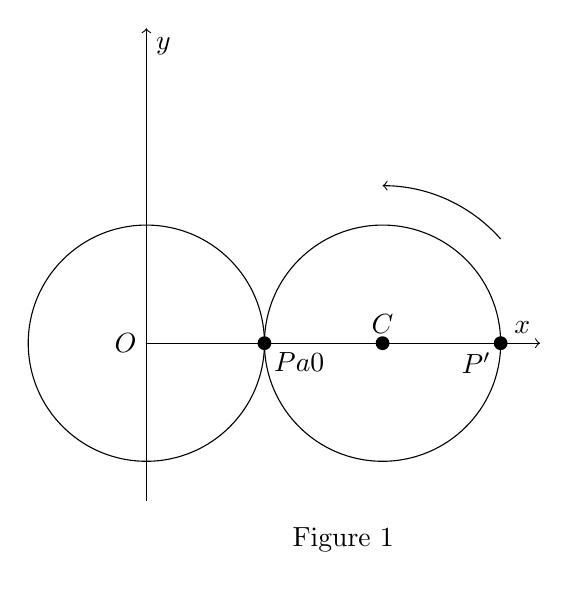
\begin{tikzpicture}
                    \coordinate[label=left:$O$] (O) at (0, 0);
                    \coordinate[label=above:$C$] (C) at (3, 0);
                    \coordinate[label=below right:$P\coord{a}0$] (P) at (1.5, 0);
                    \coordinate[label=below left:$P'$] (P') at (4.5, 0);

                    \draw[->] (0, -2) -- (0, 4) node[anchor=north west] {$y$};
                    \draw[->] (O) -- (5, 0) node[anchor=south east] {$x$};

                    \draw (O) -- (C);
                    \draw (O) circle[radius=1.5];
                    \draw (C) circle[radius=1.5];

                    \fill (C) circle[radius=2.5pt];
                    \fill (P) circle[radius=2.5pt];
                    \fill (P') circle[radius=2.5pt];

                    \draw[->] (4.5,1.323) arc[radius=2, start angle=41.4, end angle=90];

                    \node at (2.5, -2.5) {Figure 1};
                \end{tikzpicture}
            \end{center}
        \end{minipage}
        \begin{minipage}{0.45\textwidth}
            \begin{center}
                \begin{tikzpicture}
                    \coordinate[label=left:$O$] (O) at (0, 0);
                    \coordinate[label=above:$C$] (C) at (2.24, 2);
                    \coordinate[label=below right:$P\coord{x}{y}$] (P) at (2.0685, 0.5076);
                    \coordinate (X) at (1, 0);

                    \draw[->] (0, -2) -- (0, 4) node[anchor=north west] {$y$};
                    \draw[->] (O) -- (5, 0) node[anchor=south east] {$x$};

                    \draw (O) -- (C);
                    \draw (O) circle[radius=1.5];
                    \draw (C) circle[radius=1.5];

                    \fill (C) circle[radius=2.5pt];
                    \fill (P) circle[radius=2.5pt];

                    \draw[->] (4.24, 2) arc[radius=2, start angle=0, end angle=45];

                    \draw pic [draw, angle radius=9mm, "$\theta$"] {angle = X--O--C};

                    \node at (2.5, -2.5) {Figure 2};
                \end{tikzpicture}
            \end{center}
        \end{minipage}

        \begin{enumerate}
            \item Show that the equation of one full revolution of the path of $P$ can be represented by
            \begin{align*}
                x &= 2a\cos\theta - a\cos2\theta\\
                y &= 2a\sin\theta - a\sin2\theta
            \end{align*}
            \item Sketch the path of $P$ for $0 \leq \theta \leq 2\pi$, indicating clearly the coordinates of the $x$-intercepts.
            \item Without the use of a calculator, find the length of the path of $P$ in terms of $a$.
            \item A student commented that a point $P'$ with the initial position $\coord{3a}0$ (as shown in Figure 1) is further away from $O$ than point $P$ and therefore travels a longer path as the circular gear makes a full revolution around the fixed circular axle. Do you agree with the comment? Justify your answer.
        \end{enumerate}

    \solution
        \part
            \begin{center}
                \begin{tikzpicture}
                    \coordinate[label=left:$O$] (O) at (0, 0);
                    \coordinate[label=above:$C$] (C) at (4.48*5/3, 4*5/3);
                    \coordinate[label=below left:$P$] (P) at (4.137*5/3, 1.0152*5/3);
                    \coordinate (X) at (1, 0);
                    \coordinate[label=below right:$G$] (G) at (4.48*5/3, 1.0152*5/3);
                    \coordinate[label=below:$F$] (F) at (4.48*5/3, 0);
                    \coordinate[label=below:$E$] (E) at (6.707, 0);

                    \draw[->] (0, -0.5) -- (0, 7) node[anchor=north west] {$y$};
                    \draw[->] (O) -- (8.5, 0) node[anchor=south east] {$x$};

                    \clip (-0.5, -0.5) rectangle (8.5, 7);

                    \draw (O) -- (C);
                    \draw[dotted, thick] (C) -- (E);
                    \draw[dotted, thick] (C) -- (F);
                    \draw (O) circle[radius=5];
                    \draw (C) circle[radius=5];

                    \fill (C) circle[radius=2.5pt];
                    \fill (P) circle[radius=2.5pt];
                    \fill (G) circle[radius=2.5pt];
                    \fill (F) circle[radius=2.5pt];
                    \fill (E) circle[radius=2.5pt];

                    \draw pic [draw, angle radius=12mm, "$\theta$"] {angle = X--O--C};

                    \draw pic [draw, angle radius=3mm, ""] {right angle = E--F--C};
                    \draw pic [draw, angle radius=3mm, ""] {right angle = P--G--C};
                \end{tikzpicture}
            \end{center}

            \noindent Consider the above diagram. Let $E$ be the intersection between the $x$-axis and $CP$ extended. Let $F$ be the point on the $x$-axis such that $CF \perp OF$. Let $G$ be the point on the line $CF$ such that $PG \perp CG \implies PG \parallel EF$.

            By symmetry, $OE = EC$, whence $\triangle OEC$ is isoceles. Hence, $\angle COE = \angle OCE = \theta$. By the exterior angle theorem, $\angle CEF = 2\theta$. Since $PG \parallel EF$, we have $\angle CPG = \angle CEF = 2\theta$. Finally, from the angle sum of a triangle, we have $\angle ECF = \dfrac\pi2 - \theta$.
            \begin{alignat*}{8}
                &&\cos\angle COF &= \dfrac{OF}{OC} &\implies&&\cos\theta &= \dfrac{OF}{2a} &\implies &&OF &= 2a\cos\theta\\
                &&\cos \angle CPG &= \dfrac{PG}{PC} &\implies&& \cos 2\theta &= \dfrac{PG}{a} &\implies&& PG &= a\cos2\theta
            \end{alignat*}
            Since $x = OF - PG$, we have
            \begin{equation*}
                x = 2a\cos\theta - a\cos2\theta
            \end{equation*}
            \begin{alignat*}{8}
                &&\cos \angle OCF &= \dfrac{CF}{OC} &\implies&& \cos \left(\dfrac\pi2 - \theta\right) &= \dfrac{CF}{2a} &\implies&& CF &= 2a\sin\theta\\
                &&\cos \angle PCG &= \dfrac{CG}{PC} &\implies&& \cos \left(\dfrac\pi2 - 2\theta\right) &= \dfrac{CG}{a} &\implies&& CG &= a\sin2\theta
            \end{alignat*}
            Since $y = CF - CG$, we have
            \begin{equation*}
                y = 2a\sin\theta - a\sin2\theta
            \end{equation*}
            Hence, the path of $P$ can be represented by
            \begin{align*}
                x &= 2a\cos\theta - a\cos2\theta\\
                y &= 2a\sin\theta - a\sin2\theta
            \end{align*}

        \part
            \begin{alignat*}{2}
                &&r^2 &= x^2 + y^2\\
                && &= (2a\cos\theta - a\cos2\theta)^2 + (2a\sin\theta - a\sin2\theta)^2\\
                && &= a^2\Big[(2\cos\theta - \cos2\theta)^2 + (2\sin\theta - \sin2\theta)^2\Big]\\
                && &= a^2\Big[4\cos^2\theta - 4\cos\theta\cos2\theta + \cos^2 2\theta + 4\sin^2\theta - 4\sin\theta\sin2\theta + \sin^2 2\theta\Big]\\
                && &= a^2\Big[(4\cos^2\theta + 4\sin^2\theta) + (\cos^2 2\theta + \sin^2 2\theta) - 4(\cos\theta\cos2\theta + \sin\theta\sin2\theta)\Big]\\
                && &= a^2(4 + 1 - 4\cos\theta)\\
                && &= a^2 (5 - 4\cos\theta)\\
                \implies&&r &= \pm a \sqrt{5 - 4\cos\theta}
            \end{alignat*}

            \begin{center}
                \begin{tikzpicture}[trim axis left, trim axis right]
                    \begin{axis}[
                        domain = 0:2*pi,
                        samples = 100,
                        axis y line=middle,
                        axis x line=middle,
                        xtick = {-3, 1},
                        xticklabels = {$-3a$, $a$},
                        xmin=-3.5,
                        xmax=1.5,
                        ymin=-2.5,
                        ymax=2.5,
                        ytick = \empty,
                        xlabel = {$x$},
                        ylabel = {$y$},
                        legend cell align={left},
                        legend pos=outer north east,
                        after end axis/.code={
                            \path (axis cs:0,0) 
                                node [anchor=north east] {$O$};
                            }
                        ]
                        \addplot[color=plotRed,data cs=polarrad] {sqrt(5 - 4*cos(\x r))};
            
                        \addlegendentry{$r^2 = 5 - 4\cos\theta$};
                    \end{axis}
                \end{tikzpicture}
            \end{center}

        \part
            Note that we have $\der{x}{\theta} = -2a\sin\theta + 2a\sin2\theta$ and $\der{y}{\theta} = 2a\cos\theta - 2a\cos2\theta$. Thus, 
            \begin{align*}
                \left(\der{x}{\theta}\right)^2 &+ \left(\der{y}{\theta}\right)^2\\
                &= \left(-2a\sin\theta + 2a\sin2\theta\right)^2 + \left(2a\cos\theta - 2a\cos2\theta\right)^2\\
                &= 4a^2\Big[\left(-\sin\theta + \sin2\theta\right)^2 + \left(\cos\theta - \cos2\theta\right)^2\Big]\\
                &= 4a^2\Big[\sin^2\theta - 2\sin\theta\sin2\theta + \sin^2 2\theta + \cos^2\theta - 2\cos\theta\cos2\theta + \cos^2 2\theta\Big]\\
                &= 4a^2\Big[\left(\sin^2\theta + \cos^2\theta\right) + \left(\sin^2 2\theta + \cos^2 2\theta\right) - 2\left(\sin\theta\sin2\theta + \cos\theta\cos2\theta\right)\Big]\\
                &= 4a^2\left(1 + 1 - 2\cos\theta\right)\\
                &= 8a^2\left(1 - \cos\theta\right)
            \end{align*}
            Hence, the length of the path of $P$ is given by
            {\allowdisplaybreaks
            \begin{align*}
                \text{Length} &= \int_0^{2\pi} \sqrt{\left(\der{x}{\theta}\right)^2 + \left(\der{y}{\theta}\right)^2} \d \theta\\
                &= \int_0^{2\pi} \sqrt{8a^2(1 - \cos\theta)} \d \theta\\
                &= \sqrt8 a \int_0^{2\pi} \sqrt{1 - \cos\theta}\d \theta\\
                &= \sqrt8 a \int_0^{2\pi} \sqrt{2\sin^2 \left(\dfrac\theta2\right)}\d \theta\\
                &= 4 a \int_0^{2\pi} \sin \left(\dfrac\theta2\right) \d \theta \usub{u &= \theta/2\\\d u &= \d \theta/2}\\
                &= 8 a \int_0^{\pi} \sin u \d \theta\\
                &= 8 a \eval{-\cos u}{0}{\pi}\\
                &= 16a
            \end{align*}
            }

            \boxt{
                The length of the path of $P$ is $16a$ units.
            }

        \part
            When the gear has rotated $\pi$ radians, $P$ ends up at $\coord{-3a}0$. This iis the reflection of $P'$ in the $y$-axis. Indeed, $P'$ also ends up at $\coord{-a}0$, which is the reflection of $P$ in the $y$-axis. Hence, the path taken by $P'$ is excatly the path taken by $P$ in the $y$-axis, but reflected in the $y$-axis. Hence, the total length travelled by $P$ and $P'$ are equal. Thus, the comment is incorrect.

    \problem{}
        To promote Earth Day, the Earth Day Network organises an event that will be held for $n$ consecutive days. Cash prizes will be awarded to participants throughout the event, with one lucky participant chosen each day. Let the budget for the cash prizes by \$$m$.
        
        The amount of cash prize given out on the first day is a sum of \$10 and $\dfrac17$ of the remaining budget, i.e. \$$\left(10 + \dfrac17 (m - 10)\right)$. The amount of cash prize given out on the second day is a sum of \$20 and $\dfrac17$ of the remaining budget. In general, the amount of cash prize given out on the $k$th day is a sum of \$$10k$ and $\dfrac17$ of the remaining budget. Let $u_k$ denote the amount of cash prize given out on the $k$th day, with $1 \leq k \leq n$, $k \in \mathbb{Z}^+$.

        \begin{enumerate}
            \item Write down the expression for $u_k$, in terms of $u_1, u_2, \ldots, u_{k-1}$.
            \item By considering $u_{k+1} - u_k$, show that $u_{k+1} = \dfrac67 u_k + \dfrac{60}7$.
            \item Find $u_k$ in the form $u_k = p\left(\dfrac67\right)^k (m - 360) + q$, where $p$ and $q$ are constants to be determined.
        \end{enumerate}

        \noindent It is given that $m = 4000$.

        \begin{enumerate}
            \setcounter{enumi}{3}
            \item Find an expression of the total amount of cash prizes given out in $n$ days. Hence or otherwise, explain if it is possible for the Earth Day Network to host this event for 2 weeks.
            \item Find the set of values of $k$ for which the daily cash prize will be less than 5\% of the initial budget.
            \item Determine the minimum budget that the Earth Day Network needs to have so that they can host this event for 2 weeks.
        \end{enumerate}

    \solution
        \part
            On the $k$th day, the total cash prizes that have already been given out is $u_1 + u_2 + \ldots + u_{k-1}$. Hence,
            \boxt{
                $u_k = 10k + \dfrac17 \Big(m - 10k - (u_1 + u_2 + \ldots + u_{k-1})\Big)$
            }

        \part
            {\allowdisplaybreaks
            \begin{alignat*}{2}
                &&u_{k+1} - u_k &= 10(k+1) + \dfrac17 \Big(m - 10(k+1) - (u_1 + u_2 + \ldots + u_k)\Big)\\
                && &\hspace{1.8em}- \left(10k + \dfrac17 \Big(m - 10k - (u_1 + u_2 + \ldots + u_{k-1})\Big)\right)\\
                && &= 10 + \dfrac17(-10 - u_k)\\
                && &= \dfrac{60}7 - \dfrac17 u_k\\
                \implies&&u_{k+1} &= \dfrac{60}7 + \dfrac67 u_k
            \end{alignat*}
            }

        \part
            Let $x$ be the constant such that $u_k + x = \dfrac67 (u_{k-1} + x)$. Then $-\dfrac17 x = \dfrac{60}7 \implies x = -60$.
            \begin{alignat*}{2}
                &&u_k -60 &= \dfrac67 (u_{k-1} - 60)\\
                && &= \left(\dfrac67\right)^{k-1} (u_1 - 60)\\
                \implies&&u_k &= \left(\dfrac67\right)^{k-1} \left(10 + \dfrac17 (m - 10) - 60\right) + 60\\
                && &= \left(\dfrac67\right)^{k-1} \left(\dfrac17 m - \dfrac{360}7\right) + 60\\
                && &= \left(\dfrac67\right)^k \cdot \dfrac76 \left(\dfrac17 m - \dfrac{360}7\right) + 60\\
                && &= \dfrac16 \left(\dfrac67\right)^k \left( m - 360\right) + 60\\
            \end{alignat*}

            \boxt{
                $u_k = \dfrac16 \left(\dfrac67\right)^k \left( m - 360\right) + 60$
            }

        \part
            Let $S_n$ be the total amount of cash prizes given out in $n$ days.
            \begin{align*}
                S_n &= \sum_{k=1}^n u_k\\
                &= \sum_{k=1}^n \left(\dfrac16 \left(\dfrac67\right)^k \left( m - 360\right) + 60\right)\\
                &= \dfrac{m-360}6 \cdot \dfrac67 \cdot \dfrac{1 - (6/7)^n}{1 - 6/7} + 60n\\
                &= (m-360) \left(1 - \left(\dfrac67\right)^n\right) + 60n
            \end{align*}
            Substituting $m = 4000$ and $n = 14$, we have
            \begin{align*}
                S_{14} &= (4000 - 360) \left(1 - \left(\dfrac67\right)^{14}\right) + 60\cdot14\\
                &= 4059
            \end{align*}
            Since $S_{14} > 4000 = m$, there is not enough money to pay out the cash prizes for 14 days, or 2 weeks.

            \boxt{
                It is not poassible for the Earth Day Network to host this event for 2 weeks.
            }

        \part
            Consider $u_k < \dfrac5{100}m = 200$.
            \begin{alignat*}{2}
                &&u_k &< 200\\
                \implies&&\dfrac16 \left(\dfrac67\right)^k \left(4000 - 360\right) + 60 &< 200\\
                \implies&&\left(\dfrac67\right)^k &< \dfrac3{13}\\
                \implies&&k &> \log_{6/7} \dfrac3{13}\\
                && &= 9.5 \tosf{2}
            \end{alignat*}

            Note that $S_{13} = (4000 - 360) \left(1 - \left(\dfrac67\right)^{13}\right) + 60\cdot13 = 3929 < 4000 = m$. Hence,
            \boxt{
                $\{k \in \mathbb{N} : 10 \leq k \leq 13\}$
            }

        \part
            Consider $S_{14} \leq m$.
            \begin{alignat*}{2}
                &&S_{14} &\leq m\\
                \implies&&(m-360) \left(1 - \left(\dfrac67\right)^{14}\right) + 60\cdot14 &\leq m\\
                \implies&&m\left(1 - \left(\dfrac67\right)^{14}\right) - 360\left(1 - \left(\dfrac67\right)^{14}\right) + 840 &\leq m\\
                \implies&&m - m\left(\dfrac67\right)^{14} -m &\leq 360\left(1 - \left(\dfrac67\right)^{14}\right) - 840\\
                \implies&&- m\left(\dfrac67\right)^{14} &\leq 360\left(1 - \left(\dfrac67\right)^{14}\right) - 840\\
                \implies&& m &\geq \dfrac{840 - 360\left(1 - (6/7)^{14}\right)}{(6/7)^{14}}\\
                && &= 4514.285
            \end{alignat*}

            \boxt{
                Earth Day Network needs to have a minimum budget of \$$4514.29$.
            }
\end{document}